\chapter[Resultados Alcançados]{\textbf{R}esultados \textbf{A}lcançados}
\addcontentsline{toc}{chapter}{Resultados Alcançados}

\textit{Será apresentado neste capítulo a execução dos experimentos sob a solução abordada nas seções anteriores, e exposto os resultados que foram alcançados.}

\section{Hardware da implantação}

Na realização da implantação da solução proposta,  foram utilizados os seguintes recursos de hardware:

\begin{table}[htb]
	\center
	\footnotesize
	\begin{tabular}{|p{0.5cm}|p{3.5cm}|p{3cm}|p{2cm}|p{4cm}|} \hline
		\textbf{Nº} & \textbf{SISTEMA OPER.} & \textbf{PROCESSADOR} & \textbf{MEMÓRIA} & \textbf{ARMAZENAMENTO}  \\ \hline
		1 & CentOS 2.6 64 bits & Intel Core i7 & 6GB & 1TB \\ \hline
		2 & Windows 7 64 bits & Intel Core i5-3210M CPU@2.50GHz & 8GB & 300GB \\ \hline
		3 & Kali Linux 3.14 64 bits & Intel Core i7 & 2GB & 250GB \\ \hline
	\end{tabular}
\end{table}
\begin{center}
	Tabela  4 : Tabela de recursos utilizados. \\
	Fonte: Autoria Própria
\end{center}

\begin{description}
	\item O recurso de número 1 é responsável em executar o software Asterisk paralelamente com Middleware desenvolvido, tornando o Call Center disponível a chamadas via VoIP.
	\item O recurso de número 2 é responsável em executar o sistema GSAN através do servidor de aplicação Jboss 4.1,  juntamente com o banco de dados Postgres.
	\item O recurso de número 3 é responsável em simular chamadas VoIP para o Call Center (Asterisk).	
\end{description}

Ambos os recursos estão conectados a uma rede local distribuída por um switch DLink 501, dessa forma cada recurso pode ser acessível na rede local. A rede local permite conexões de até 300 Mb/s conforme a especificação do Switch utilizado.


\section{Estabelecer Métricas}
De forma geral as companhias de saneamento atendem diariamente um acentuado volume de reclamações e solicitações de serviços a serem prestados, sejam para execução de serviços internos como serviços a serem prestados fora do ambiente da empresa, que normalmente exige um maior tempo para solucionar o atendimento.
Neste trabalho foi definida a média de atendimento dos principais tipos de serviços disponíveis no sistema GSAN específicos para o módulo Atendimento ao Público que são registrados diariamente, com base em informações obtidas através de relatórios regulatórios e entrevistas com funcionários da Companhia de Sanaeamento Manaus Ambiental, acerca dos atendimentos prestados nas Centrais de Atendimentos das empresas de saneamento, com base em análise das reclamações por tipos de serviço, foi construído o seguinte gráfico, conforme demonstrado na figura \ref{figura:mediaAtendimentos} abaixo:

\begin{figure}[!htb]
	\centering
	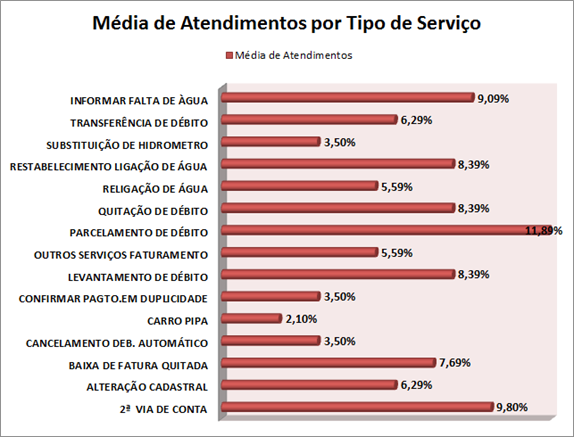
\includegraphics{figuras/media_atendimentos.png}
	\caption{Média de atendimentos diários em companhias de saneamento}	
	\label{figura:mediaAtendimentos}
	Fonte – Autoria Própria
\end{figure}


% TODO: Dúvida sobre a palavra Call Center no plural :D
Com base na média de atendimentos realizados por tipos de serviços exposto acima, notamos que os serviços automatizados propostos neste trabalho representam o total de 27,28\% dos atendimentos prestados diariamente nas centrais de atendimentos das companhias de saneamento, no entanto para que seja possível atender plenamente essa parcela dos atendimentos, foram propostos cenários de teste para averiguar o quão eficiente à solução está em solucionar os cenários.




\section{Cenários de Testes}

Os cenários de testes representam as possíveis situações cadastrais ou comportamentais apresentadas pelo cliente ao longo do atendimento, onde cada cenário deve ser totalmente atendimento para que se tenha êxito no atendimento e posteriormente a situação de \textbf{ATENDINDO}, caso contrário será obtido à situação de \textbf{NÃO ATENDINDO}, caso o atendimento não seja concluído com sucesso o cenário deve conter uma observação, descrevendo o motivo ao qual levou a tal situação.
Abaixo serão descritos os Cenários dos serviços propostos:

\subsection{Obter 2ª Via de Conta}
Abaixo serão descritos os casos de testes previstos para o serviço Obter 2ª Via de Conta;
\begin{flushleft}
\begin{description}
\item \textbf{CENÁRIO 1}: Cliente devidamente cadastrado no Sistema, atualmente proprietário de um único imóvel que possui ativo a Ligação de Água e Esgoto, com pendência de duas contas. O Cliente deseja obter as duas contas em aberto.
\item \textbf{SITUAÇÃO}: ATENDINDO
\item \textbf{OBSERVAÇÃO}: Não aplicável
\end{description}

\begin{description}
\item \textbf{CENÁRIO 2}: Cliente devidamente cadastrado no Sistema, atualmente sendo usuário de um imóvel que possui a Ligação de Água cortada por falta de pagamento, atualmente com quatro contas em aberto. O Cliente deseja obter as quatro contas em aberto.
\item \textbf{SITUAÇÃO}: ATENDINDO
\item \textbf{OBSERVAÇÃO}: Não aplicável
\end{description}

\begin{description}
\item \textbf{CENÁRIO 3}: Cliente devidamente cadastrado no Sistema, atualmente sendo responsável por três imóveis que possuem ativo a Ligação de Água e Esgoto, possuindo uma conta pendente para cada imóvel. O Cliente pretende obter a conta pendente de somente um imóvel específico. 
\item \textbf{SITUAÇÃO}: ATENDINDO
\item \textbf{OBSERVAÇÃO}: Não aplicável
\end{description}

\begin{description}
\item \textbf{CENÁRIO 4}: Cliente sem e-mail cadastrado no Sistema, atualmente sendo responsável por dois imóveis que possuem ativo a Ligação de Água e Esgoto, possuindo duas contas pendente para cada imóvel.  O cliente pretende obter todas a contas em aberto dos dois imóveis. 
\item \textbf{SITUAÇÃO}: NÃO ATENDINDO
\item \textbf{OBSERVAÇÃO}: Devido a falta do e-mail no cadastro do cliente não será possível enviar as contas pendentes ao mesmo, e também a solução inicialmente está tratando dos débitos de um imóvel por vez, sendo necessário redirecionar a ligação para o atendente concluir o atendimento, ou repetir a operação.
\end{description}
\end{flushleft}


\subsection{Informar Falta de Água}
Abaixo serão descritos os casos de testes previstos para o serviço Informar Falta de Água;
\begin{flushleft}
\begin{description}
	\item \textbf{CENÁRIO 1}: Cliente devidamente cadastrado no Sistema, atualmente proprietário de um único imóvel que possui ativo a Ligação de Água e Esgoto, com pendência de duas contas, com problemas no abastecimento de água. O Cliente pretende informar a falta de água para o único imóvel.
	\item \textbf{SITUAÇÃO}: ATENDINDO
	\item \textbf{OBSERVAÇÃO}: Não aplicável
\end{description}
\begin{description}
	\item \textbf{CENÁRIO 2}: Cliente sem e-mail cadastrado no Sistema, atualmente usuário de um único imóvel que possui ativo a Ligação de Água, com situação de adimplência, com problemas no abastecimento de água. O Cliente pretende informar a falta de água para o único imóvel.
	\item \textbf{SITUAÇÃO}: ATENDINDO
	\item \textbf{OBSERVAÇÃO}: Não aplicável
\end{description}
\begin{description}
	\item \textbf{CENÁRIO 3}: Cliente devidamente cadastrado no Sistema, atualmente responsável por três imóveis que possuem ativo a Ligação de Água, com uma conta pendente para cada imóvel. O Cliente deseja informar problemas no abastecimento de água para um imóvel específico ao qual o mesmo é responsável.
	\item \textbf{SITUAÇÃO}: ATENDINDO
	\item \textbf{OBSERVAÇÃO}: Não aplicável
\end{description}
\begin{description}
	\item \textbf{CENÁRIO 4}: Cliente devidamente cadastrado no Sistema, atualmente responsável por dois imóveis em locais diferentes, que possuem a Ligação de Água ativa, em recente situação de adimplência. O Cliente deseja informar problemas no abastecimento de água para os dois imóveis ao qual o mesmo é responsável.
	\item \textbf{SITUAÇÃO}: NÃO ATENDINDO
	\item \textbf{OBSERVAÇÃO}: A solução inicialmente para Informar Falta de Água está tratando apenas um imóvel por vez, sendo necessário redirecionar a ligação para o atendente concluir o atendimento, ou repetir a operação.
\end{description}
\end{flushleft}	

\subsection{Solicitar Restabelecimento da Ligação de Água}
Abaixo serão descritos os casos de testes previstos para o serviço Solicitar Restabelecimento da Ligação de Água;
\begin{flushleft}
\begin{description}
	\item \textbf{CENÁRIO 1}: Cliente devidamente cadastrado no Sistema, atualmente proprietário de um único imóvel que possui a Ligação de Água interrompida por corte, em situação recente de adimplência. O Cliente deseja solicitar restabelecimento da ligação para o imóvel.
	\item \textbf{SITUAÇÃO}: ATENDINDO
	\item \textbf{OBSERVAÇÃO}: Não aplicável
\end{description}
\begin{description}
	\item \textbf{CENÁRIO 2}: Cliente devidamente cadastrado no Sistema, atualmente usuário de um único imóvel que possui a Ligação de Água interrompida por corte, em situação recente de adimplência. O Cliente deseja solicitar restabelecimento da ligação para o imóvel.
	\item \textbf{SITUAÇÃO}: ATENDINDO
	\item \textbf{OBSERVAÇÃO}: Não aplicável
\end{description}
\begin{description}
	\item \textbf{CENÁRIO 3}: Cliente devidamente cadastrado no Sistema, atualmente responsável por dois imóveis, que possuem a Ligação de Água interrompida por corte, devido a falta de pagamento das dez contas em aberto para ambos. O Cliente deseja solicitar restabelecimento da ligação para os imóveis após realizar a negociação das faturas.
	\item \textbf{SITUAÇÃO}: NÃO ATENDINDO
	\item \textbf{OBSERVAÇÃO}: A solução inicialmente está tratando o restabelecimento da ligação de apenas um imóvel por vez, sendo necessário redirecionar a ligação para o atendente concluir o atendimento, ou repetir a operação.
\end{description}

\begin{description}
	\item \textbf{CENÁRIO 4}: Cliente com cadastrado incompleto no Sistema, atualmente proprietário de um único imóvel que possui a Ligação de Água interrompida por corte, em situação recente de adimplência. O Cliente deseja solicitar restabelecimento da ligação para o imóvel.
	\item \textbf{SITUAÇÃO}: ATENDINDO
	\item \textbf{OBSERVAÇÃO}: Não aplicável	
\end{description}
\end{flushleft}	

